\section{Introduction}

% 第一段直接介绍transformer for RL 很好， 但是xx，需要in-context RL。 第二段再介绍in-context RL 然后介绍有problem
Large transformer models \cite{4} have shown impressive abilities across a variety of domains, including text \cite{5}, image \cite{6}, and audio \cite{7}. 
In the field of reinforcement learning (RL), large transformer models can treat the RL tasks as a type of sequential prediction problem, which has proven successful in using solely offline training \cite{14,27}.
A notable shortcoming lies with these methods to self-improve when employed in online environments. To overcome this, in-context RL methods have been introduced, which enable continued policy improvement \cite{8}.

% 要先强调现在性能已经很好了，再说现在的efficiency不太行。
Recent works demonstrated that in-context RL can automatically improve its performance in a trial-and-error manner when across-episodic contexts serve as prompt conditions \cite{3}. The construction of the across-episodic context is flexible and easy to implement, such as a chain of experience that consists of multiple historical trajectories arranged in ascending order of returns \cite{1}. Despite the progress made, current methods are mostly limited to short-horizon tasks with less than 100 timesteps \cite{8}. This arises from (1) the quadratic complexity of the self-attention mechanism and (2) the significant increase in the length of sequences caused by across-episodic contexts. Such huge computational costs severely limit in-context RL to apply the trial-and-error ability on traditional RL tasks, which often reach 1000 timesteps, such as MuJoCo \cite{13} and Atari \cite{15}.
% However, both reasons are indispensable to the in-context RL methods, which makes them difficult to apply to traditional RL tasks \cite{8}, such as Gym-MuJoCo \cite{13} and Atari \cite{15}.
% Due to the strict computational requirements, a key question arises:
% \begin{center}
%    \emph{How does a human do trial-and-error on \\ long-horizon tasks?} 
% \end{center}

% 这第一句话，search and memory是RL介绍那本书的第30页提到的   psychologist Edward Thorndike
% 先psychologist提出了trial-and-error，再被作为central idea of RL. 
In fact, trial-and-error is the central idea of modern RL algorithms \cite{16}. It is an animal behavior originated by a psychologist \citet{17} who considers trial-and-error as an elementary way of combining search and memory. Correspondingly, the across-episodic contexts provide memory, and the self-attention mechanism reviews historical actions in the memory to search for better actions. However, human decision-making is more complex and operates on multiple levels of temporal abstraction \cite{12}. For example, travelers tend to decide on their budget first, then their mode of transportation, right down to the smallest action. Inspired by this idea, a natural perspective emerges: 
\vspace{-5pt}
\begin{center}
\emph{``Can human multi-level decision-making bring out a more efficient trial-and-error?"}
\end{center}
\vspace{-5pt}
% {\centering\textit{``Can human multi-level decision-making bring out a more efficient trial-and-error?"}}
% Correspondingly, the across-episodic contexts provide memory, and the self-attention mechanism provides a combined way to search for better actions.
% 这句话可以放到related work中。concept-level的follow up由上边的例子引出来。
% Based on this idea, hierarchical RL proposes the high- and low-level action structure, which is more efficient in long-horizon tasks \cite{10}.
% Correspondingly, the across-episodic context contains past memory and, combined with the self-attention mechanism, provides a similar way to search better actions.
% In fact, the trial-and-error ability is one of people's strengths because people are good at reviewing their past actions and rethinking to do better.
% This concept is called temporal abstraction, which is commonly used in hierarchical RL \cite{10}. For the sake of simplicity, we refer to the temporal abstraction as ``plan'' in this paper, as shown in Figure~\ref{motivation}.
% plan这个词可能不合适，

% Since simulating human decision-making can improve the learning efficiency of RL algorithms, can the trial-and-error ability emerged from in-context RL be benefited ?
% We think .  first second xx让他看起来更像是自己的意思。 这段里最好强调出来 in-context RL中实现hierarchical有难点。
% 这段还是要先show一下1999年的概念很好但是在这里有很多问题。
% 尽量控制在三行，太长了。

% \setlength{\belowcaptionskip}{-0.3cm} %调整图片标题与下文距离 
% \setlength{\abovecaptionskip}{-0.2cm} %调整图片标题与图距离
\begin{figure}
    \centering
    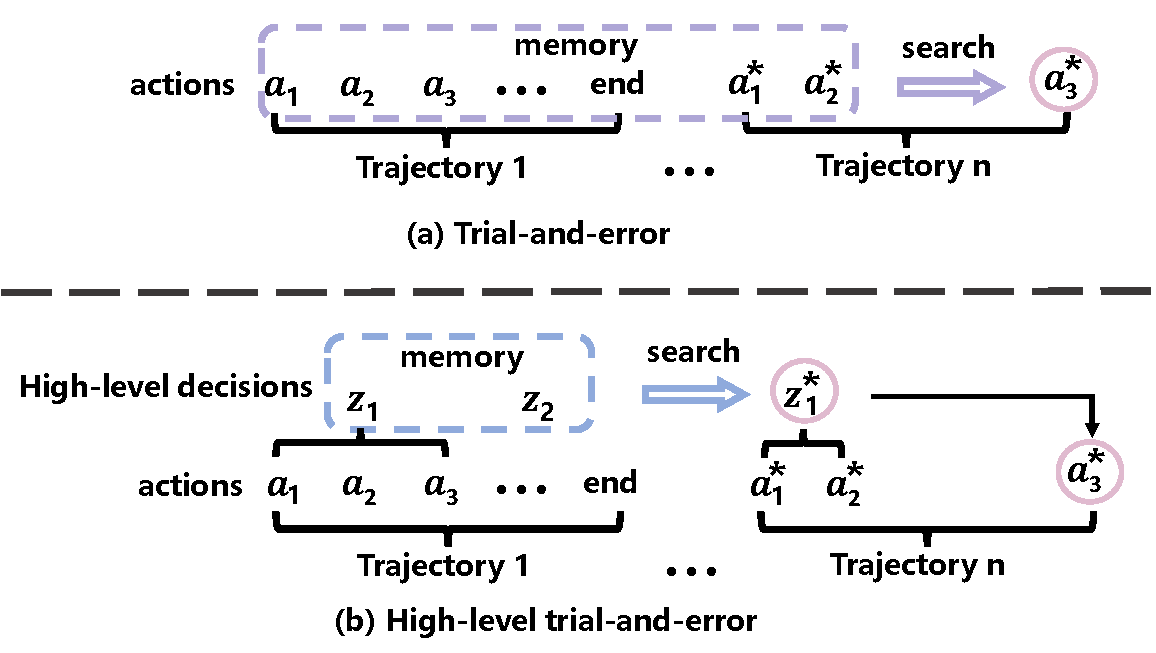
\includegraphics[width=1.0\columnwidth]{results/motivation.pdf}
    \caption{Trial-and-error comparison of minimal actions and high-level decisions, where * denotes better results. (a) In the trial-and-error process, the memory consists of the smallest actions from experiences and serves as context to search for better action. (b) In the high-level trial-and-error process, the memory and search act on high-level decisions. Since one high-level decision controls multiple actions, we can use smaller memory to preserve experiences and search for better decisions with less computational costs.}
    \label{motivation}
\end{figure}

As one high-level decision can guide multi-step low-level actions, it can considerably shorten across-episodic contexts and, therefore, significantly alleviate the computational costs. In this view, we aim to explore a high-level trial-and-error process, as shown in Figure~\ref{motivation}. 
However, since the model generates high-level decisions rather than low-level actions that interact with the environment, our first challenge is ensuring that better high-level decisions can encourage better low-level actions.
In addition, the in-context RL is trained with supervised losses, which predicts each next step conditioned on the past steps in the sequence.
Unlike low-level actions, the high-level decision is an abstract concept that is usually not directly observable from training data.
% However, the in-context RL relies on a conditional generated model that output labels for each timestep in the sequence are necessary during training.

% To this end, we propose an efficient in-context RL method called Hierarchical Chain of experience Context (H2C). 
To this end, we propose an efficient in-context RL method called In-context Decision Transformer (IDT). 
Specifically, IDT consists of Making Decisions, Decisions to Go, and Reviewing Decisions modules to mimic the high-level trial-and-error process. First, the Making Decisions module is a decoder-only transformer that generates high-level decisions autoregressively, where the high-level decision is represented by a vector sampled from a multivariate Gaussian distribution. Then, the generated high-level decisions are fed to the Decisions to Go module, which is also a decoder-only transformer to generate low-level actions autoregressively. 
The output of the Making Decisions module serves as a conditional input to the Decisions to Go module, ensuring high-level decisions correctly guide low-level actions.
To fill in the missing high-level decisions in the training data, we designed the Reviewing Decisions module to encode high-level decisions from sequences of low-level actions.
All three modules are learned end-to-end by predicting the low-level actions from the training data.
% Combining these two modules achieves the search part in the high-level trial-and-error process.
% As the high-level decisions induce low-level actions, the low-level actions should be able to infer high-level decisions inversely.

Our contributions are as follows: (1) We propose IDT, an in-context RL method that emerges with high-level trial-and-error ability. IDT can learn by directly combining sub-optimal data and efficiently improving itself through multiple trials at test time. (2) Compared to the contexts consisting of the smallest actions, IDT significantly shortens the evaluation time by \textbf{36$\bm\times$} times on the D4RL baselines \cite{13} and \textbf{27$\bm\times$} times on the Large Grid World environments \cite{14}. 
(3) IDT can achieve state-of-the-art results with less training costs, especially outstanding in long-horizon tasks. 

% Our experiments show that H2C achieves state-of-the-art results, especially outstanding in long-horizon tasks. 


% 这里不要引用一篇论文。要体现a series of work。
% H2C incorporates high-level decisions into the chain of hindsight experience \cite{1} that consists of multiple trajectories arranged in ascending order of total rewards.
% The ``Making Decisions" module is a decoder-only transformer to predict a high-level decision, which is represented by a multivariate Gaussian distribution.
% Then, the ``Decisions to Go" module is also a decoder-only transformer to predict actions based on the high-level decision, where one high-level decision serves as multi-step actions. Finally, the ``Reviewing Decisions" module is an encoder to review the high-level decision and serve as contexts to predict the next high-level decision. 
% In particular, the ``Reviewing Decisions" module can not only encode replays from the ``Decisions to Go" module but also encode expert trajectories to solve unseen tasks more quickly.

% In the field of reinforcement learning (RL), large transformer models can treat the RL tasks as a type of sequential prediction problem and complete it through in-context learning, referred to as in-context RL \cite{8}.
% Equipped with the trial-and-error ability, in-context RL could quickly adapt to unseen tasks without computationally expensive gradient-based optimizing.
% across-episodic context c
% Large transformer models \cite{4} have shown impressive abilities to achieve complex tasks given input contexts, with applications extending across multiple domains like text \cite{5}, image \cite{6}, and audio \cite{7}.
% Recent work demonstrated that reinforcement learning (RL) tasks can be treated as a type of sequential prediction problem and utilize large transformer models to achieve complex tasks through in-context learning, referred to as in-context RL \cite{8}.
% After modeling the reinforcement learning (RL) as a sequential prediction problem, large transformer models have been shown to adapt to downstream tasks through in-context learning, referred to as in-context RL \cite{8}.
% In the field of reinforcement learning (RL), recent works have proven successful in tackling unseen tasks when across-episodic contexts serve as prompts, referred to as in-context RL .
% well-trained large transformer model 改成in-context RL. in-context RL大于trial-and-error. 
% For instance, a well-trained large transformer model can emerge with the trial-and-error ability to predict better actions when input conditions are multiple historical trajectories arranged in ascending order of returns.
% Equipped with the trial-and-error ability, the transformer model could quickly adapt to unseen tasks by providing across-episodic contexts without computationally expensive gradient-based optimizing.

% In the field of reinforcement learning (RL), recent works have proven successful in tackling unseen tasks when conditioning on across-episodic contexts, referred to as in-context RL \cite{8}.
% Large transformer models \cite{4} have shown impressive abilities to perform tasks \jf{achieve difficult tasks} given input contexts, with applications extending across multiple domains like text \cite{5}, image \cite{6}, and audio \cite{7}. In the field of reinforcement learning (RL), recent work has \jf{recent works have} proven successful in tackling unseen tasks when treating state-action-reward tuples as context, referred to as in-context RL \cite{8} \jf{suggest use 'In-context RL'}. For instance, a well-trained large transformer model can emerge with trial-and-error abilities to predict better actions when input conditions are across-episodic contexts, i.e., multiple trajectories from the learning history \jf{historical trajectory interactions} of RL algorithms. Compared with fine-tuning methods \cite{9}\jf{never see 'fine-tuning methods' before, so you should introduce what is 'fine-tuning methods'}, in-context RL could quickly adapt to unseen tasks through inference alone \jf{the reason should be illustrated. Besides, 'inference alone' also needs to be illustrated.}.

% A trial-and-error process arising from inference alone is appealing but often requires large-scale RL learning trajectories from diverse tasks, which brings enormous training costs \cite{1}.
% To promote the application of in-context RL, \citet{1} introduced the return-to-go method \cite{2} into the context, using suboptimal trajectories more efficiently. With a similar purpose, \citet{3} proposed predicting only optimal actions from in-context interactions and theoretically proven that this produces a sample-efficient Bayesian RL algorithm.
% \jf{Generally, these sentences are more similar to 'related work' rather than 'introduction'. Can we separate the in-context RL into several classes? then introduce}

% During the trial-and-error process, the high-level decision is critical because it is not only related to the quality of low-level executed action but also serves as the experience of subsequent decision.
% Inspired by the hierarchical structure, we explore to realize a high-level trial-and-error ability on the in-context RL. 

% According to the way humans make decisions, the trial-and-error process can be seen as three stages: (1) making a plan, (2) executing the plan, and (3) reviewing the plan. Among the three stages, making plans is a crucial step throughout the trial-and-error process because it is not only related to the quality of executed action but also serves as the experience of subsequent planning. Inspired by this idea, the across-episodic contexts can be designed at the plan level instead of the smallest actions. Since the plan is a high-level temporal abstraction, it can greatly shorten the length of contexts and significantly alleviate the computational complexity of the self-attention mechanism.
% making better plans is the key to the trial-and-error process, which means that this stage is the most likely to require across-episodic contexts.
% Since planning is a high-level temporal abstraction, it can greatly shorten the length of trajectories. Compared with the smallest action, across-episodic context and self-attention mechanism will further amplify the advantages of plans and significantly alleviate the computational complexity.


% In fact, in-context RL is designed to mimic the way humans think. \jf{since you have introduced 'humans think', why you do not introduce more about 'humans think' successively? for example, you introduce 'human will think 'across-episodic context' before decision', then the 'across-episodic context' will relate to the next sentence.} Since the across-episodic context contains several historical explorations of the task, it provides a hindsight method to predict better behaviors. However, instead of reviewing every step, humans review at a high level of time abstraction. \jf{emmmm, maybe 'high level of time abstraction' is a little abstract. Besides, I think you should implicitly mention 'hierarchical' before you introduce 'hierarchical RL' so as to make readers agree with your intuition.} Inspired by the idea of hierarchical RL \cite{10}, we refer to the time abstraction as the ``plan" in this paper. Therefore, we can divide the human trial-and-error process into three stages: (1) making a plan, (2) executing the plan, and (3) hindsight \jf{too short}. Among the three stages, making better plans is the key to the trial-and-error process, which means that this stage may be the most likely to require across-episodic contexts. Since planning is a high-level temporal abstraction, it can greatly shorten the context length and significantly alleviate the computational complexity during training and inference. \jf{from 'high time abstraction' I can imagine 'short context length', but you should say more clearly about the reason of 'alleviate the computational complexity'.}

% H2C relies on the chain of hindsight experience \cite{1}, which uses return-to-go as a template to build context by arranging multiple trajectories with ascending returns.
% At inference time, the ``Plans hindsight" module can not only be used to encode its own replays, but also encode expert trajectories like the prompt decision transformer method \cite{11} to solve unseen tasks directly.

% Inspired by the success of the hierarchical structure, we aim to explore a more efficient trial-and-error process by introducing high-level decisions.
% During the trial-and-error process, the high-level decision plays an important role that is closely connected with search and memory, as shown in Figure ~\ref{motivation}. 
% A high-level decision is generated from the search process and directly affects the quality of low-level executed actions. Subsequently, it also serves as the memory for future searches.
% In addition, one high-level decision guides multiple steps of low-level actions, which can considerably shorten the length of contexts and significantly alleviate the computational complexity of the self-attention mechanism. 
% Therefore, we suggest the trial-and-error process on high-level decisions instead of the smallest actions.